\section{Platforms and tools for refactoring}
\subsubsection{Language Server Protocol} \label{sec:lsp}
The \ac{LSP}  \cite{lsp_website} is a protocol developed by Microsoft to create a language-independent interface for code-related operations. 
The \ac{LSP}  describes a server and a client who communicate to each other using the JSON-Remote-Process-Call protocol \cite{json_rpc}. 

The client can generally be anything that works with source code but has no detailed knowledge of a specific programming language. For instance, an \ac{IDE}, an editor or a refactoring tool can be described as a client.

The client starts a server based on a programming language. The server has a inherent knowledge of one ore more programming languages and can provide source-code-related functionality. For instance, the server can rename a variable, find the usages of a method, or inform the client about compiler errors. 

Initially, client and server share some information to set up. This includes the path to the project that the server should load and information about what functionality each of them supports. These functionalities are named \textit{Capabilities}. For example, the server can announce that it supports renaming variables while the client is capable of showing error messages. Hence, server and client can interact in a manner such that no unsupported messages are transferred.

The sequence diagram in figure \ref{fig:lsp_usage} illustrates how the \ac{LSP} works in practice after the initialization process. 
\begin{figure}
    \centering
    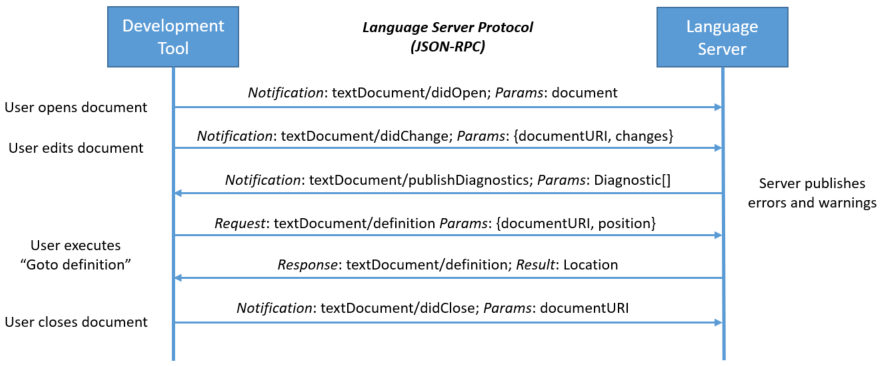
\includegraphics{figures/chapter2/language-server-sequence.png}
    \caption{Example usage of the Language Server Protocol}
    \label{fig:lsp_usage}
    \cite{lsp_website}
\end{figure}

After the server has been successfully started by the client, a user can open a document (e.g. source code file). The request to open the document is submitted to the server. From now one, the server may not rely on the file system since that might be not the current version of the opened document. 

The client can now inform the server about some changes (e.g. adding a new method). The server can, in the meantime, inform the client about syntactical errors which the client might show to the user of the client.

Afterward, the client requests the definition of a method or variable, and the server returns a response with the requested data.

In the end, the client can save the document and notify the server that the document was closed which means that the physical file of the document represents the current version of the document again. 

The \ac{LSP} can hence be used to simplify refactoring-related task. For instance, a mandatory part of refactoring is to find all references of a symbol (e.~g. variable). The \ac{LSP} can perform this step so that the detected references can be processed further. It should however be noted that functionality of the protocol is limited to maximize the support for many programming languages. Thus, the an \ac{LSP} server is not a refactoring tool per-se. 





\subsubsection{Data clump doctor} \label{sec:data_clump_doctor}

The  \textit{DataClumpDoctor} is NodeJS command line tool developed by Nils Baumgartner  to detect data clumps. It employs \textit{PMD} to find all classes, methods, and fields in a Java project to generate an \ac{AST}. Each Java file is converted to an \ac{AST} that does not contain the bodies of methods or documentation.

In a second step, the generated \ac{AST} can be loaded again to find data clumps. by using the algorithmic approach discussed in section \ref{sec:data_clump_detection}. With this two-step methodology, a greater programming language independence can be achieved as the data clump detection does not need access to the original source code. The \textit{DataClumpDoctor} reports its result in the format discussed in appendix \ref{sec:data_clump_format}

For purposes of this master thesis, the results from the \textit{DataClumpDoctor} are treated as the ground truth with regard to data clump detection. 

\subsubsection{ Program Structure Interface}\label{sec:psi}
The Program Structure Interface provided by IntelliJ is an \ac{API} to analyze and modify  projects that the \ac{IDE} \textit{IntelliJ} can load. As a result, the various classes, methods etc. can be obtained which allows for the detection of data clumps. Also modifications are possible which makes it a suitable candidate for refactoring purposes.

In order to use this API, an instance of IntelliJ must be started. IntelliJ can be started in a headless mode to reduce loading times and improve the performance so that no GUI is initialized. Nevertheless, IntelliJ requires many resources and much overhead, so that  the initialization needs some time.


\section{Related work}\label{sec:related_research}


The code smell \enquote{data clumps} has been the focus of multiple papers and several tools were developed for detecting and refactoring data clumps. However, none of them performs fully automatic refactoring and integrates \acp{LLM}.
Since the surge of large language models is fairly recent, many novel papers attempt to analyze their usefulness for code generation and refactoring tasks.

\subsubsection{Related to data clumps}

As outlined in section \ref{sec:data_clump_def}, the definition of data clump by Fowler \cite{fowler2019refactoring} is somewhat ambiguous because no clear criteria to determine data clumps is established. Zang et al. \cite{zhangImprovingPrecisionFowler2008} creates a more algorithmic approach to determine whether a data clump exists. This approach is also explained in section \ref{sec:data_clump_def}. The authors also provide more precise definitions of other code smells like \enquote{message chains} or \enquote{speculative generality}. By interviewing four software development experts about the code smell definitions the authors developed, they find that their new data clump definition receives relatively more disagreement than other definitions, which the authors explain are the results of not covering edge cases in the definitions. 


Hall et al. analyzed the impact of code smells (including data clump) on the occurrence of faults in three open-source software projects. They find that data clumps have a mixed correlation to faults because, in two of the three projects analyzed, the correlation of data clumps per \ac{LOC} to detected faults is negative for two projects and positive for one project. This rejects their hypothesis that data clumps do not affect faults, and the authors suggest that the application domain and the development context need to be considered before the time-consuming refactoring of data clumps since their impact is not predictable.  \cite{hallCodeSmellsHave2014}


Baumgartner et al. developed a live code smell detection plugin for IntelliJ that can detect, report, and refactor data clumps without significantly impacting performance. However, the tool is semi-automatic, meaning the developer must still actively approve the data clump refactoring and suggest a suitable class name for the extracted class. \cite{BaumgartnerAP23}

Murphy et al. \cite{stench_blossom} developed a visual tool to find code smells (including data clumps). the tool named \textit{Stench Blossom} is a plugin for Eclipse. If a plugin user views a file, the tool searches for code smells and displays them at the right side of the eclipse editor. Each code smell is visually displayed as a a \textbf{petal}. The radius of such petal represents the strength of a smell (i.~e. how strongly violates the code smell the given coding guidelines). The petal has a color that indicates how obvious a code smell is. Orange code smells are not very obvious while blue code smells are easy to detect by human beings. Since orange has a closer connection to warnings, it is more easily to perceive so that undetected code smells can be fixed better. Experiments with \textit{Stench Blossom} shows that the median number of code smells detected by humans using the tool increased from 11 to 21. However, data particular for data clumps is not given.




\subsubsection{Related to large language models in software development}

White et al. \cite{White2023ChatGPTPP} outline how ChatGPT can be used in software development to improve the worklflow of developers. This includes  exploration of requirements, removing ambiguity in technical specification, or describing source code. The authors suggest specific prompts to elicit a suitable response from ChatGPt.

In case of refactoring, the author suggest that ChatGPT is able to refactor code with multiple prompts. For instance, ChatGPT can refactor based on a well known design pattern name, multiple examples on how to refactor the code, or a more lengthy requirements description. The exact success of each prompt is however dependent on how ChatGPT is trained and should be scrutinized manually. 

Cao et al. \cite{cao2023study} focus on using ChatGPT for fixing deep learning programs. Those are programs that cannot be understood only by their source code alone, but are are largely influenced by underlying data like  neural networks etc. This makes finding faults more difficult. The study finds out that ChatGPT can find code smells and detect faults. Without giving instructions however, ChatGPT will tend to return code smells and outdated API calls while not finding other bugs. 


Madaan et al. present a self-refinement process for \acp{LLM} with regard to code generation. Their idea is to submit the output of a model to the model again so the code can be evaluated by the model. The feedback returned by the \ac{LLM} is the used to improve the code again so as long as a stop condition is reached. They find that this approach increases the quality of the generated code. For instance, the number of optimized programs using this strategy increases from 27.3~\% to 36~\%. \cite{Madaan2023SelfRefineIR}. 
The general idea of this approach will also be used in this master thesis to correct building errors that can occur after using an \ac{LLM}. 
